As pygrace is still young, the only method yet available to install it
is to download the source code from:

\begin{command}
http://sourceforge.net/projects/pygrace
\end{command}

\noindent
The subsection titled \textit{Installing a development version}
describes how to download the source code.

\subsection*{Installing a development version}

\begin{flushleft}

To check out the pygrace repository, change to a directory where you
want to put pygrace, and type:

\begin{command}
svn co https://pygrace.svn.sourceforge.net/svnroot/pygrace/trunk
pygrace
\end{command}

\begin{figure}[t!]
  \centering
  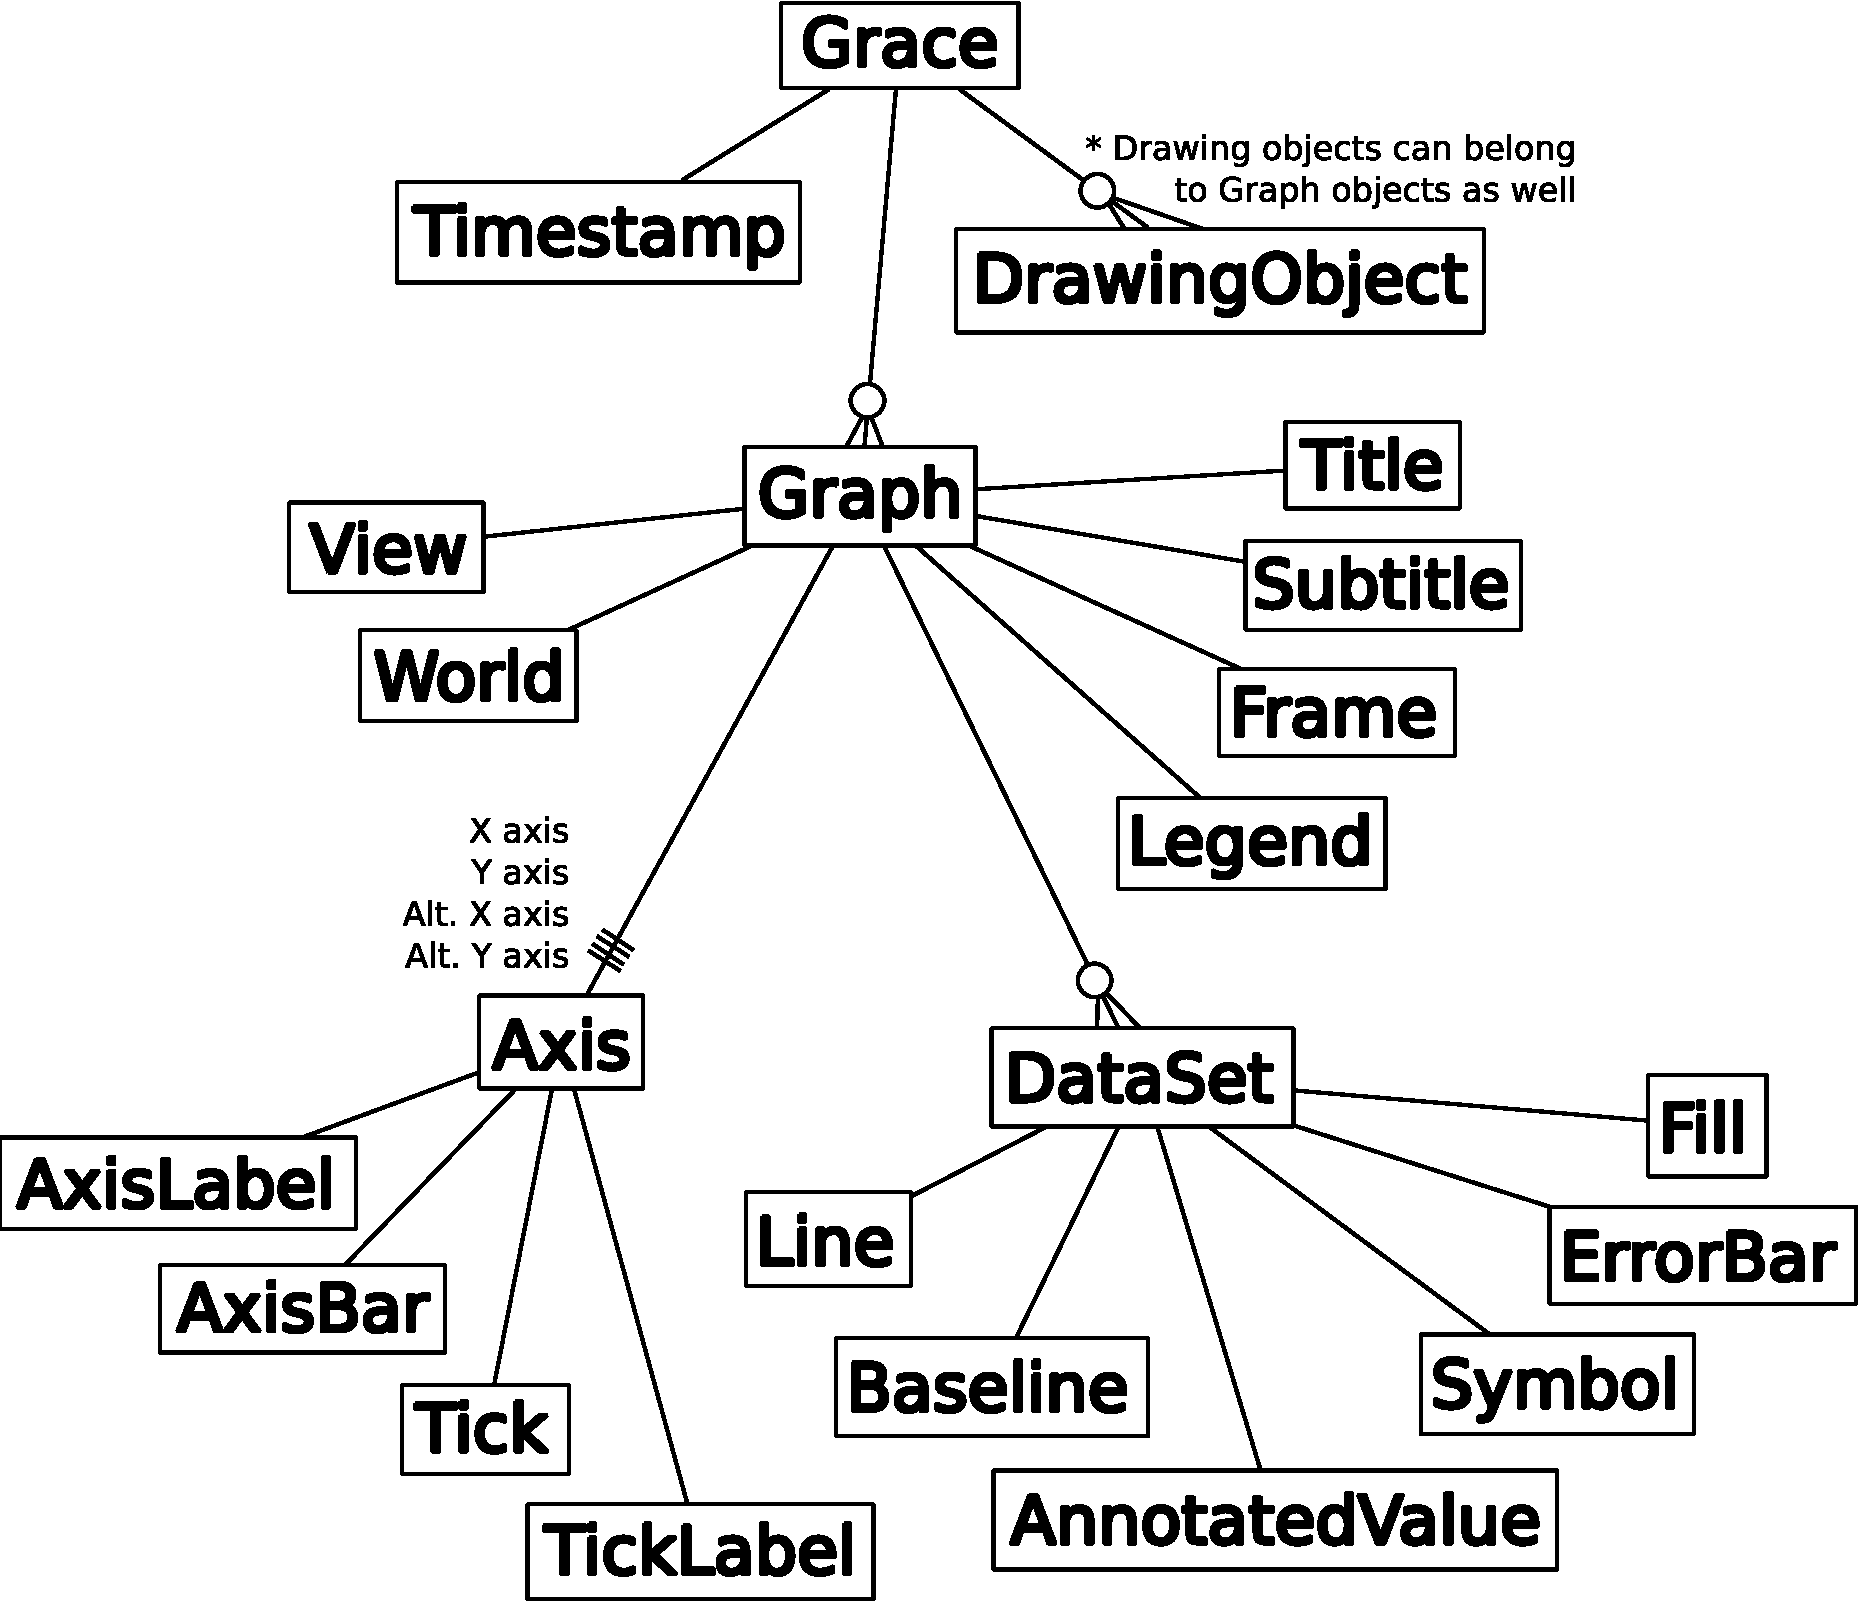
\includegraphics[width=0.67\textwidth]{../Diagrams/crow_diagram.pdf}
  \caption{
%
The inheritance structure of pygrace mirrors the file structure of
Grace.  This diagram uses ``crow's foot'' notation to indicate the
relationship between different entities.
%
  }
  \label{crowdiagram}
\end{figure}

Install pygrace (to python's site-packages directory):

\begin{command}
python setup.py install
\end{command}

This will put pygrace on the {\tt PYTHONPATH}, so import statement
in python scripts can find the pygrace library.

You can test that pygrace was installed corrctly by opening
an interactive python prompt and typing:

\begin{command}
import pygrace
\end{command}

If no error is raised, then installation was succesful!

\end{flushleft}
